\documentclass[tikz,border=8pt]{standalone}
\usetikzlibrary{arrows.meta,positioning}
\begin{document}
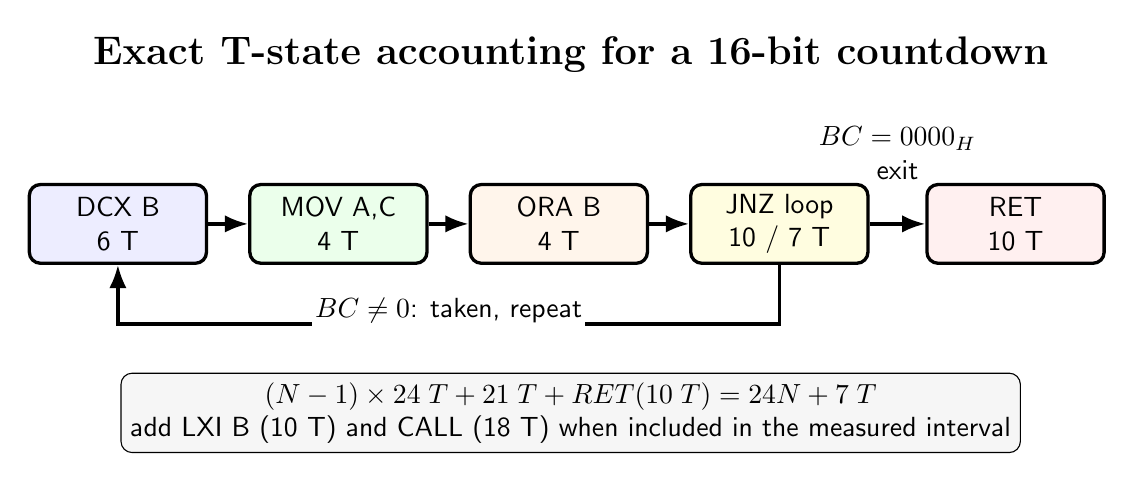
\begin{tikzpicture}[font=\sffamily,>=Latex,
 op/.style={draw,very thick,rounded corners,minimum width=2.25cm,minimum height=1cm,align=center}]
\node[font=\Large\bfseries] at (7.0,5.6) {Exact T-state accounting for a 16-bit countdown};
\node[op,fill=blue!7] (dcx) at (1.25,3.45) {DCX B\\6 T};
\node[op,fill=green!8] (mov) at (4.05,3.45) {MOV A,C\\4 T};
\node[op,fill=orange!8] (ora) at (6.85,3.45) {ORA B\\4 T};
\node[op,fill=yellow!12] (jnz) at (9.65,3.45) {JNZ loop\\10 / 7 T};
\node[op,fill=red!6] (ret) at (12.65,3.45) {RET\\10 T};
\foreach \a/\b in {dcx/mov,mov/ora,ora/jnz}{\draw[very thick,->] (\a)--(\b);}
\draw[very thick,->] (jnz)--(ret);
\node[align=center] at (11.15,4.35) {$BC=0000_H$\\exit};
\draw[very thick,->] (jnz.south)--++(0,-.75)-|(dcx.south);
\node[fill=white,inner sep=1pt] at (5.45,2.35) {$BC\ne0$: taken, repeat};
\node[draw,rounded corners,fill=gray!7,align=center,minimum width=11cm] at (7.0,1.05) {$(N-1)\times24\;T + 21\;T + RET(10\;T)=24N+7\;T$\\add LXI B (10 T) and CALL (18 T) when included in the measured interval};
\end{tikzpicture}
\end{document}
